\externaldocument{GEP/deliverable1.tex}

\section{Integración de OmpSs-2 en C/C++ COMPSs}

Con tal de realizar una buena integración necesitamos conocer bien cómo funcionan y/o cómo están hechos los componentes a integrar. Con tal de adquirir los conocimientos necesarios, vamos a indagar en la estructura interna del \textit{binding} de \textit{C/C++} de \textit{COMPSs} y a entender cómo se desarrolla y compila una aplicación. También deberemos ver cómo funciona la \textit{API} del \textit{runtime} de \textit{OmpSs-2} \textit{Nanos6} y el proceso habitual de desarrollo y compilado de una aplicación que utiliza el modo librería.

\subsection{Estructura de los bindings}

El \textit{runtime} de \textit{COMPSs} fue desarrollado en \textit{Java}, por lo que si queremos soportar cualquier lenguaje (salvo el propio \textit{Java}), necesitamos de alguna manera establecer comunicación con ese lenguaje. Es decir, necesitaremos un mecanismo que nos permita ejecutar código de este lenguaje a soportar, por supuesto, en ambas direcciones. 
\par\bigskip
Actualmente, \textit{COMPSs} cuenta con los \textit{bindings} de \textit{C/C++} y \textit{Python} (usualmente conocido como \textit{PyCOMPSs}), que utilizan estos mecanismos descritos anteriormente. Para efectuar la ejecución entre \textit{Java} y \textit{C/C++} se utiliza la \textit{Java Native Interface}, dado que desde \textit{Python} se puede utilizar la \textit{Python-C API} para , con un componente intermedio entre \textit{Python} y \textit{Java} escrito en \textit{C/C++} (utilizando la \textit{JNI}) permitiríamos efectuar llamadas desde \textit{C/C++} y \textit{Python} al \textit{runtime} y al revés. 
\par\bigskip
La siguiente imagen muestra la estructura general de los \textit{bindings} actuales. Las cajas representan componentes de la arquitectura, el color de cada caja ha sido escogido para representar un lenguaje, por lo que dos cajas del mismo color que estén conectadas directamente con un flecha no requieren de mecanismos adicionales.

\begin{figure}[H]
    \centering 
    \caption{Estructura de los bindings de COMPSs.}
    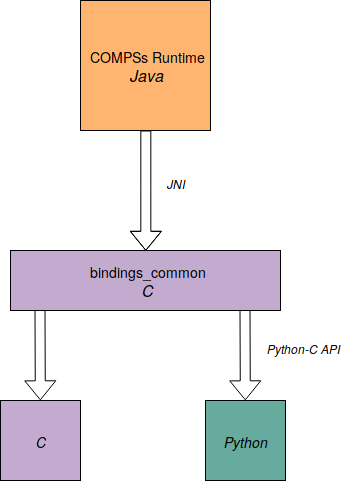
\includegraphics[scale=0.6]{estructuraBindings.png}
    \label{fig:estructurabindings}
\end{figure}

\subsection{Modelo de ejecución en el binding C/C++}
\label{sec:bindings}

Para poder obtener el modelo de ejecución introducido en la sección \ref{modeloejecucion}, necesitaremos compilar dos binarios, uno para el \textit{master} y otro para los \textit{workers}.
\par\bigskip

La aplicación que desarrolle el usuario, tiene que ser transparente al \textit{runtime}, se necesita una interfaz indicando las tareas a detectar al ejecutar la aplicación. Entonces, una vez la compilemos, se generará automáticamente (a partir de ahora \textit{autogenerar}) código para las tareas, que gestionarán la comunicación con el \textit{runtime}.
\smallskip
La siguiente imagen describe de manera visual cómo se compila una aplicación. 

\begin{figure}[H]
    \centering 
    \caption{Proceso de compilación de una aplicación COMPSs C/C++.}
    %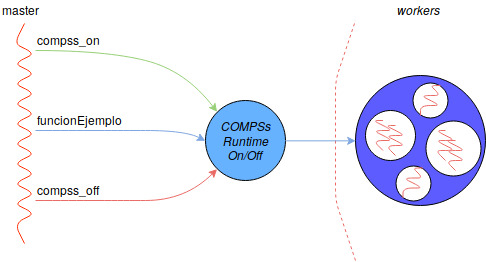
\includegraphics[width=\textwidth]{sta-masterworker.jpg}
    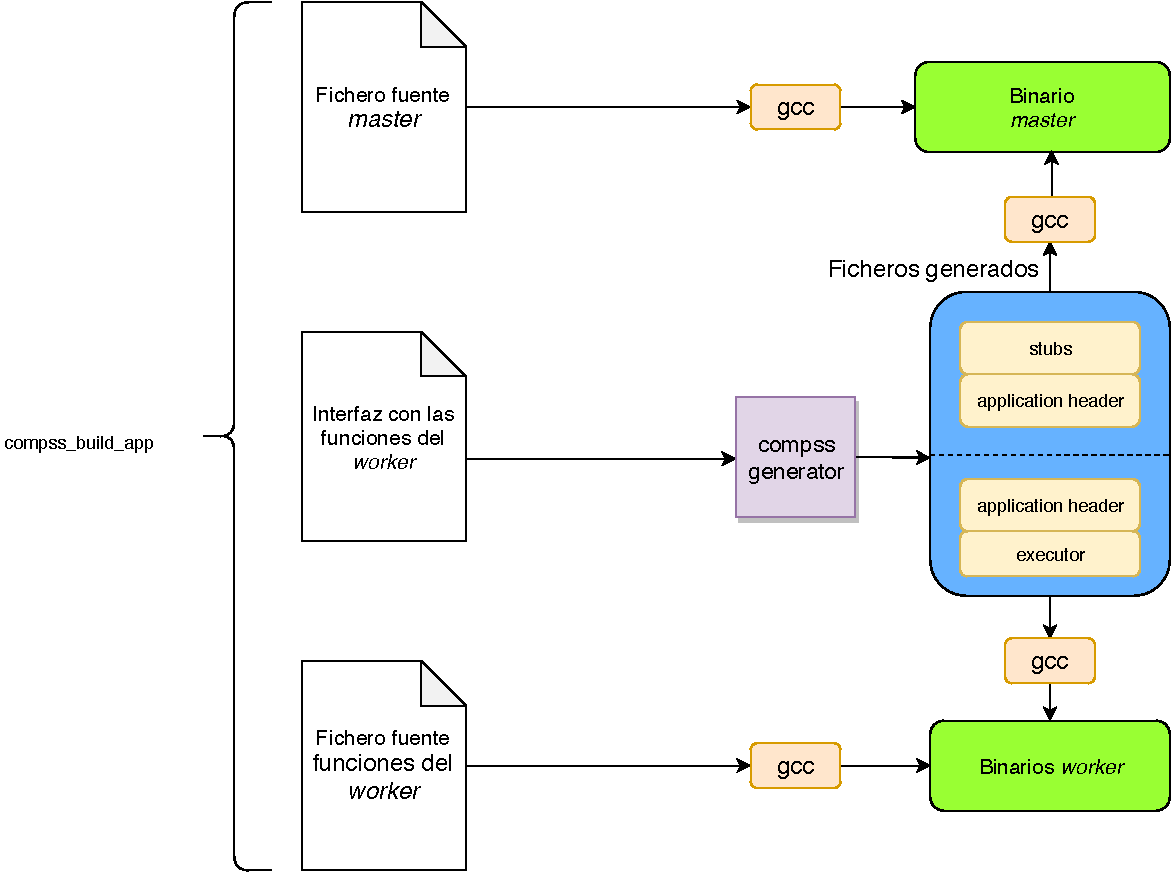
\includegraphics[scale=0.7]{workflowComp.pdf}
    \label{fig:workflowcompilado}
\end{figure}

\par\bigskip
Para facilitar el compilado de la aplicación se utiliza el script \textit{compss\_build\_app}, y para hacer la generación de código a partir de la interfaz, el binario \textit{compss\_generator}.
La aplicación una vez desarrollada por el usuario, compilada sin \textit{COMPSs} por el medio también funcionaría, pero sencillamente las tareas serían ejecutadas \textit{in situ} en el \textit{master}.  Lo que pretendemos hacer al introducir \textit{COMPSs} es que el \textit{master}, en vez de ejecutar la tarea, comunique al \textit{runtime} que se debe ejecutar una tarea, y este se encargue de ejecutarla en un \textit{worker}, todo de manera transparente al usuario.

\par\bigskip
En la figura \ref{fig:workflowcompilado} aparecen los ficheros generados con \textit{compss\_generator} y la interfaz, estos ficheros son el \textit{stubs} y \textit{executor} (siempre del estilo, \textit{ejemplo-stubs.cc} y \textit{ejemplo-executor.cc} donde ejemplo es el nombre de la aplicación compilada). El fichero \textit{stubs} corresponde con la parte del \textit{master} que se encargará de comunicarse con el \textit{runtime} para registrar la tarea. Esto lo consigue implementando las funciones de las tareas con el código para gestionar su registro, es decir, sustituyendo el código que sería propio de la ejecución de cada tarea por un código para efectuar el registro en el \textit{runtime}. Una vez registrada la tarea, eventualmente el \textit{runtime} designará a un \textit{worker} a ejecutarla. El \textit{worker} recibirá la tarea que debe ejecutar, los datos necesarios y más parámetros, el \textit{executor} ha sido \textit{autogenerado} con el código principal de la aplicación, por lo que conoce como gestionar los datos y parámetros recibidos para ejecutar la tarea pertinente. 

\subsection{Modo librería: nanos6\_spawn\_function \label{spawnfunction}}

En la sección \ref{sec:bindings} dimos una visión más interna y propia de desarrollador del \textit{binding} de \textit{C/C++}. Sobre \textit{OmpSs-2} necesitamos saber, como se desarrolla una aplicación, en concreto con el modo librería.
\medskip

Esta funcionalidad, nos permite registrar una tarea en el \textit{runtime} de \textit{OmpSs-2} de manera asíncrona, con lo cuál podremos brindar a cada tarea y sus sucesoras un entorno aislado del resto. Gracias a esto, conseguiremos arreglar el problema con la migración de \textit{threads}. \smallskip

\begin{minipage}{\linewidth}
\begin{lstlisting}[caption={Definición de la función nanos6\_spawn\_function.},captionpos=b, label={lst:nanos6spawn}, language=C++]
void nanos6_spawn_function(
   void (*function)(void *), 
   void *args,
   void (*completion_callback)(void *), 
   void *completion_args, 
   char const *label
);
\end{lstlisting}
\end{minipage}

La anterior imagen muestra la definición de la función que nos permitirá registrar una función \textbf{function} con argumentos \textbf{args} en el \textit{runtime}. Una vez ejecutada la función registrada como tarea, se ejecutará la función \textbf{completion\_callback} con argumentos \textbf{completion\_args} (mecanismo conocido como \textit{callback}, de ahí el nombre), el argumento de la función \textit{label} sirve para etiquetar la tarea con el nombre que contenga.

\subsubsection{Ejemplo}
\label{sec:ejemplo}

Con tal de entender como funciona un programa que utilice el modo librería, vamos a ver un ejemplo sencillo. Este programa de ejemplo, hará \textit{spawn} de una función y dentro de ésta se generarán tareas con dependencias entre ellas. \smallskip

\begin{minipage}{\linewidth}
\begin{lstlisting} [caption={Función a ser registrada como tarea.},captionpos=b, label={lst:nanos6ejemplo}, language=C++]
 int nanos6_ejemplo(int* a) {

    int local_a;

    #pragma oss task shared(local_a) out(local_a) 
    {
        local_a = a[0];
    }

    #pragma oss task shared(local_a) inout(local_a)
    {
        local_a = local_a * 4;
    }

    #pragma oss taskwait

    return local_a;
}
\end{lstlisting}
\end{minipage}

En la imagen podemos ver la función \textbf{nanos6\_ejemplo}, ésta tiene como parámetro un puntero a enteros \textbf{a} y retorna un valor del tipo \textbf{int}. La función será registrada como tarea desde otro fichero. El cálculo que se realiza en la función no tiene la menor importancia, es solo un \textbf{ejemplo}. \medskip

Por supuesto, esta función será compilada con \textit{Mercurium}, si no fuera el caso, la función se ejecutaría correctamente pero no se generarían las tareas de dentro de la función, por lo cuál la ejecución sería secuencial. 

\begin{minipage}{\linewidth}
\begin{lstlisting} [caption={Gestión del modo librería desde el main.},captionpos=b, label={lst:library-main}, language=C++]
    char const *error = nanos6_library_mode_init();
    if (error != NULL)
    {
        fprintf(stderr, "Error initializing Nanos6: %s\n", error);
        return 1;
    }

    condition_variable_t cond_var = COND_VAR_INIT;

    ejemplo_wrapper_args_t args;

    int A = 1;
    args.array = &A;
    
    nanos6_spawn_function(nanos6_wrapper, &args, 
    					  condition_variable_callback, &cond_var, 
    					  "spawned ejemplo");

    wait_condition_variable(&cond_var);

    printf("%li\n", args.ret);

    nanos6_shutdown();

\end{lstlisting}
\end{minipage}

Las funciones \textit{nanos6\_library\_mode\_init()} y \textit{nanos6\_shutdown()} efectúan respectivamente el encendido y apagado del \textit{runtime}, el código que vemos entre estas dos llamadas es el correspondiente para registrar una función como tarea utilizando el modo librería. Dado que la función nanos6\_spawn\_function espera como un puntero los parámetros a pasar a la función, se deben incluir todos dentro de una estructura que los pueda contener, el \textit{struct} \textit{ejemplo\_wrapper\_args\_t} tiene los campos \textbf{a} y \textbf{ret} que corresponden al parámetro de la función \textit{nanos6\_ejemplo} y valor de retorno de ésta.

\par\bigskip
Un detalle que no se ha comentado es que la ejecución de este código será efectuada por \textit{pthreads}, el estándar \textit{POSIX} de \textit{threads}. Dado que la ejecución de la tarea tendrá lugar de manera \textbf{asíncrona} es necesario un mecanismo de sincronización, la implementación de \textit{threads} que utilizamos (y por tanto los mecanismos de sincronización dependerán de estos).

\par\bigskip

Requerimos de un mecanismo de sincronización por que la función que se registra como tarea la ejecuta un \textit{thread} diferente al que la registra, se hace uso de la librería \textit{pthread} \ref{appendix:pthread}.
\par\bigskip

\begin{comment}
\begin{figure}[H]
    \centering 
    \caption{Mecanismo de sincronización abstracto.}
    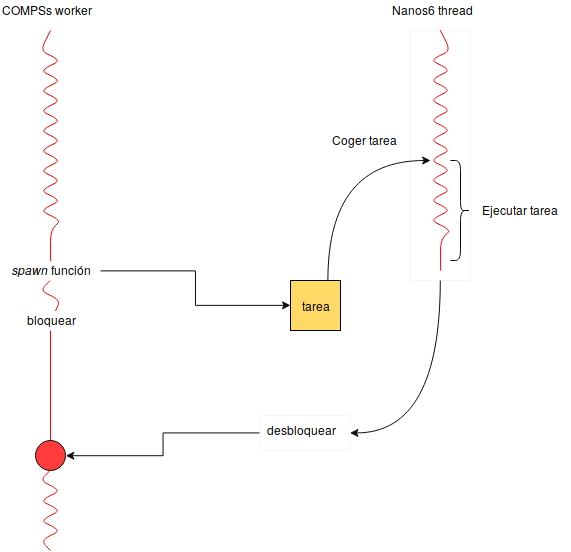
\includegraphics[scale=0.6]{spawn_sync.png}
    \label{fig:spawn\_sync}
\end{figure}
\end{comment}
 
\subsubsection{Mecanismo de sincronización} 
\label{sec:mecanismosync} 
Un \textit{thread} perteneciente al \textit{worker} de \textit{COMPSs} registra una tarea y un segundo thread perteneciente a \textit{OmpSs-2} espera a poder ejecutar alguna tarea. El primer \textit{thread} una vez haya registrado la tarea procederá a bloquearse, el segundo cuando acabe de ejecutar la tarea registrada, ejecutará un \textit{callback} donde desbloquearemos al primer \textit{thread}. \par\bigskip

El mecanismo abstracto es sencillo, pero la implementación real depende de los \textit{Pthreads}. Las estructuras utilizadas para realizar la sincronización son \textit{mutexes} y \textit{condition variables}. Un \textit{mutex} es una estructura que sirve para definir regiones de exclusión mútua mediante métodos de adquisición y liberación de la región, en este mecanismo se utilizan tan sólo por que son necesarios para utilizar \textit{condition variables}. Las \textit{condition variables} nos permiten que un \textit{thread} espere a un evento de manera no bloqueante, si no, habría que hacer \textit{polling} y consumir tiempo de cómputo inútilmente.
\par\bigskip

Será con las funciones \textit{pthread\_cond\_wait(pthread\_cond\_t * cond, pthread\_mutex\_t * mutex)} y \textit{pthread\_cond\_signal(pthread\_cond\_t * cond)} con las que respectivamente bloqueemos al primer \textit{thread} después de registrar la tarea y lo desbloqueemos al acabar de ejecutarla.
\par\bigskip

Dado que para utilizar \textit{condition variables} se necesitan \textit{mutexes} y se recomienda utilizar una variable auxiliar para evitar abrazos mortales (en el caso de que, el segundo \textit{thread} ya ha intentado desbloquear al primero, pero este aún no se había bloqueado, cuando se bloquee, se bloqueará para siempre), se crea una estructura de datos para contener todas estas variables llamada \textit{condition\_variable\_t}.

\smallskip

\begin{minipage}{\linewidth}
\begin{lstlisting} [caption={Definición de la estructura de datos condition\_variable\_t.},captionpos=b, label={lst:structwait-condition}, language=C++]
typedef struct {
    pthread_mutex_t _mutex;
    pthread_cond_t _cond;
    int _signaled;
} condition_variable_t;
\end{lstlisting}
\end{minipage}

\smallskip

\begin{minipage}{\linewidth}
\begin{lstlisting} [caption={Función wait\_condition\_variable},captionpos=b, label={lst:wait-condition}, language=C++]
void wait_condition_variable(condition_variable_t *cond_var)
{
    pthread_mutex_lock(&cond_var->_mutex);
    while (cond_var->_signaled == 0) {
        pthread_cond_wait(&cond_var->_cond, &cond_var->_mutex);
    }
    pthread_mutex_unlock(&cond_var->_mutex);
}
\end{lstlisting}
\end{minipage}

En la imagen \ref{lst:library-main} se utiliza la función \textit{wait\_condition\_variable(\&cond\_var)}, la llamada a  \textit{pthread\_cond\_wait} está dentro de una región crítica para prevenir que nadie más se bloquee sobre la misma \textit{condition variable} y esta se encuentra dentro de un \textit{while} por que puede ocurrir que el \textit{thread} se desbloquee sin haber sido desbloqueado por otro \textit{thread}, la variable \textit{cond\_var->\_signaled} será 0 hasta que el \textit{thread} que produzca el desbloqueo lo modifique, así garantizaremos que el desbloqueo es intencionado.
\smallskip

\begin{minipage}{\linewidth}
\begin{lstlisting} [caption={Callback de la tarea registrada},captionpos=b, label={lst:signal-condition}, language=C++]
void condition_variable_callback(void *untyped_arg)
{
    condition_variable_t *cond_var = (condition_variable_t *) 
    								 untyped_arg;

    pthread_mutex_lock(&cond_var->_mutex);
    cond_var->_signaled = 1;
    pthread_cond_signal(&cond_var->_cond);
    pthread_mutex_unlock(&cond_var->_mutex);
}
\end{lstlisting}
\end{minipage}

La imagen anterior muestra el \textit{callback} que se ejecuta al finalizar la ejecución de la tarea, modifica el valor de la variable \textit{cond\_var->\_signaled} y efectúa un \textit{pthread\_cond\_signal} para despertar al primer \textit{thread}.

\par\bigskip

Como es necesario utilizar una estructura auxiliar para pasar los parámetros mediante un puntero, necesitaremos también una función intermedia con la cuál llamar a la función que realmente queremos registrar como tarea. Habitualmente a este tipo de funciones intermedias se les llama \textit{wrapper}. En la siguiente imagen veremos la función que actúa como \textit{wrapper} de la función \textit{nanos6\_ejemplo}. \smallskip

\begin{minipage}{\linewidth}
\begin{lstlisting} [caption={Wrapper de la función nanos6\_ejemplo.},captionpos=b, label={lst:library-wrapper}, language=C++]
 void ejemplo_wrapper(void *untyped_arg)
{
    ejemplo_wrapper_args_t *args = 
        (ejemplo_wrapper_args_t *) untyped_arg;
    args->ret = nanos6_ejemplo(args->a);
}
\end{lstlisting}
\end{minipage}

El puntero de tipo \textit{void} puede contener cualquier tipo de estructura, aprovechando que sabemos que únicamente deberá contener el tipo \textit{ejemplo\_wrapper\_args\_t} se hace un \textit{cast} para interpretarlo como la estructura deseada. Se asigna \textbf{ret} al valor de retorno y se pasa \textbf{a} como parámetro.

\subsubsection{Compilado}
\label{sec:compilado}

El modo librería nos permite desacoplar de alguna manera la parte que pertenece a \textit{OmpSs-2} de la que no. Es decir, ahora podemos tener un código principal encargado de hacer \textit{spawn} de funciones que no tiene por qué estar compilado con \textit{Mercurium} y el \textit{flag} \textit{-{}-ompss-2}.
\par\bigskip

Un \textit{Makefile} para compilar el ejemplo \ref{sec:ejemplo} sería:
\medskip

\begin{minipage}{\linewidth}
\begin{lstlisting} [caption={Makefile para compilar el ejemplo.},captionpos=b, label={lst:makefileejemplo}, language=C++]                                                                                                                                               
all: ejemplo

# Codigo principal
main-ejemplo.o : main-ejemplo.c nanos6-ejemplo.h nanos6-helpers.h                                                                                                                                       
    $(CC) $(CFLAGS) -c main-ejemplo.c -o $@                                                                                                                                                                 

# Mecanismos de sincronizacion
nanos6-helpers.o : nanos6-helpers.c nanos6-helpers.h
    $(CC) $(CFLAGS) -c nanos6-helpers.c -o $@                                                                                                                                                                 

# Nanos6 (codigo a compilar con Mercurium y ompss-2)
nanos6-ejemplo.o :  nanos6-ejemplo.c nanos6-ejemplo.h
    $(MCC) $(CFLAGS) -c  nanos6-ejemplo.c -o $@                                                                                                                                                             

# Linking
ejemplo: main-ejemplo.o nanos6-ejemplo.o nanos6-ejemplo.o                                                                                                                                      
    $(CC) $^ -o $@ $(LIBS)                                                                                                                                                                                    
\end{lstlisting}
\end{minipage}

Se divide el \textit{Makefile} en cuatro etapas, la primera compila el \textit{main-ejemplo.c} utilizando el compilador definido por la variable de entorno \textit{CC}, en nuestro caso será \textit{g++}, la segunda etapa compila las funciones utilizadas para los mecanismos de sincronización descritos anteriormente en el fichero \textit{main-helpers.c}, la tercera compila el código que contiene la o las funciones a ser ejecutadas como tarea con el compilador definido por la variable de entorno \textit{MCC}, que es \textit{Mercurium}, y por último en una fase de \textit{linking} se enlazan los objetos compilados entre sí, y además con el objeto \textit{nanos6-library-mode.o} y la librería \textit{nanos6}, esto es necesario por que el objeto generado al compilar el \textit{main-ejemplo.c} utiliza las llamadas para encender el modo librería descritas en la sección \ref{sec:ejemplo}.

\subsection{Integración}

Con todo lo que se ha explicado acerca de \textit{OmpSs-2} y la funcionalidad del modo librería, se puede realizar la integración, esta sección muestra la forma final que han tomado los componentes al hacer la integración. Una vez realizada la integración, el proceso de compilación es el de la imagen \ref{fig:workflowcompintegration}.

\begin{figure}[H]
	\centering 
	\caption{Proceso de compilación de una aplicación COMPSs+OmpSs-2 C/C++.}
	%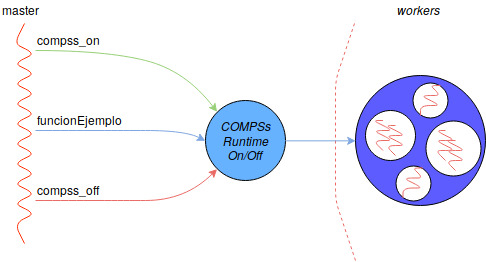
\includegraphics[width=\textwidth]{sta-masterworker.jpg}
	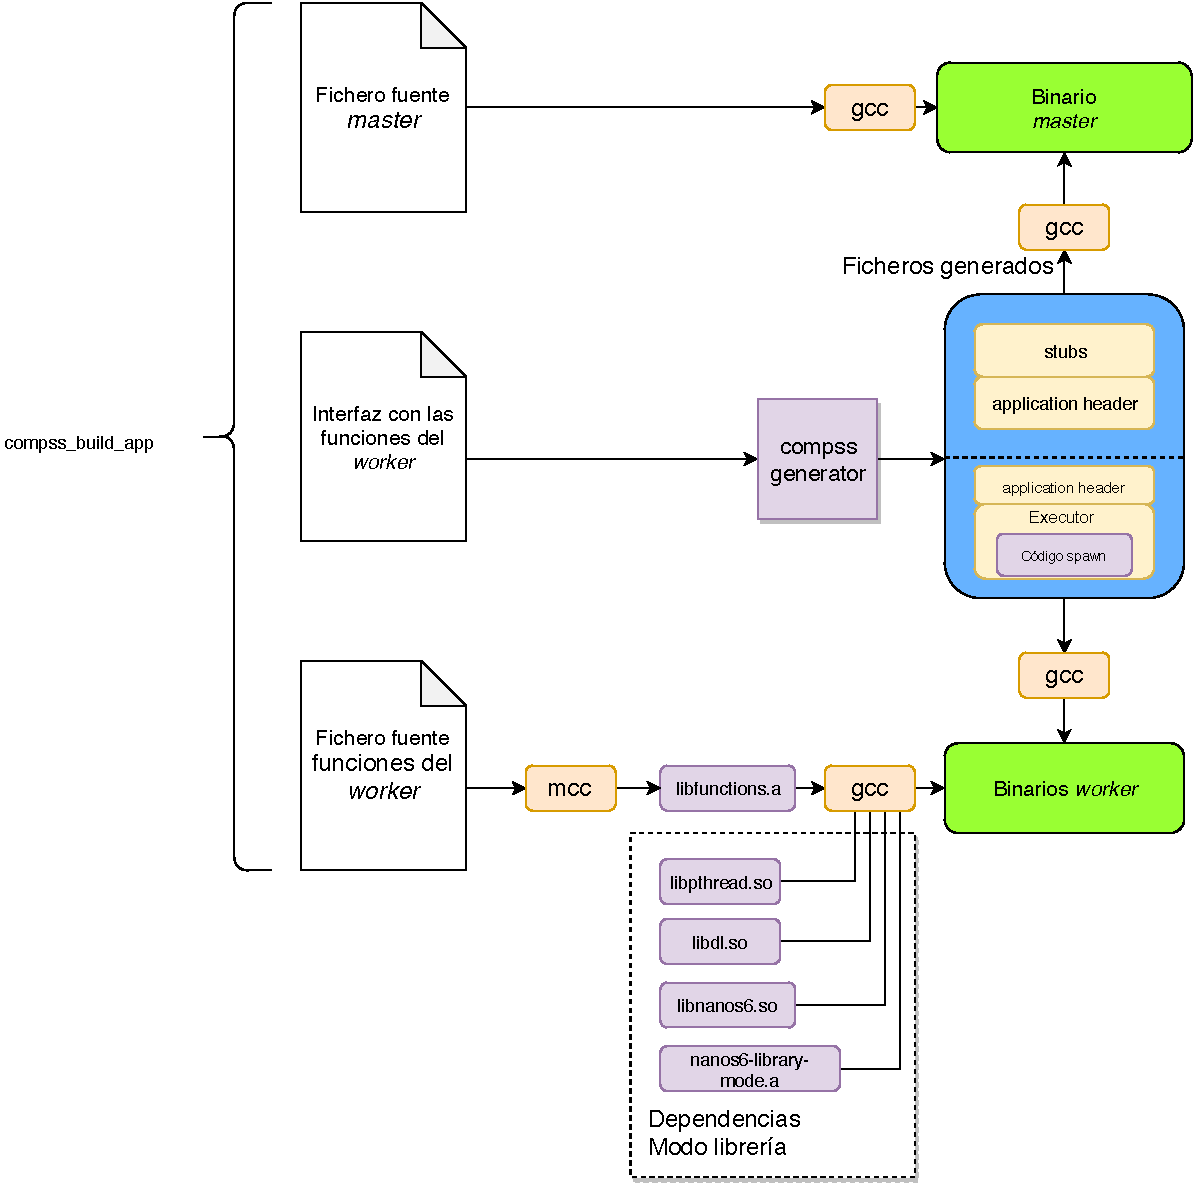
\includegraphics[scale=0.7]{workflowCompIntegration.pdf}
	\label{fig:workflowcompintegration}
\end{figure}

\par\bigskip

La única parte de toda la aplicación que hay que compilar con \textit{Mercurium} y el \textit{flag} \textit{-{}-ompss-2} es el fichero fuente que contiene las funciones del \textit{worker}. Con este fichero crearemos una librería que llamaremos \textit{libfunctions.a}, conjuntamente con las dependencias del modo librería de \textit{OmpSs-2} y los ficheros autogenerados para el \textit{worker} se compilarán los binarios \textit{worker\_c} y \textit{nio\_worker\_c}. El resto de binarios, objetos y librerías se pueden compilar con \textit{gcc} o cualquier otro compilador, esto hace mucho más flexible todo el proceso de compilado de una aplicación \textit{COMPSs+OmpSs-2}.
\par\bigskip
El nuevo proceso de compilado mantiene las características del anterior ya que genera los mismos binarios que antes y pasa por etapas similares para compilarlos, de esta manera la ejecución de una aplicación se lleva a cabo como antes. Hemos hecho la integración \textit{COMPSs+OmpSs-2} de manera transparente al resto de componentes, lo cuál es muy positivo.
\par\bigskip 

En el ejemplo para utilizar el modo librería \ref{spawnfunction}, aprendimos como activar el \textit{runtime} de \textit{OmpSs-2} en este modo y como ejecutar las tareas, por lo que bastará con activarlo en los \textit{workers} (persistente y no persistente) y modificar la generación del código \textit{executor} (queremos hacerlo en el \textit{worker}) para generar la misma estructura del ejemplo en cada tarea de la interfaz de la aplicación. En la imagen \ref{fig:genexecutorOmpSs2} se ve de manera visual lo que vimos en la sección \ref{spawnfunction} aplicado para la integración, se omiten las funciones para el mecanismo de sincronización ya que son siempre las mismas.
\bigskip
\begin{figure}[H]
	\centering 
	\caption{Generación del código para ejecutar las tareas de COMPSs en OmpSs-2.}
	%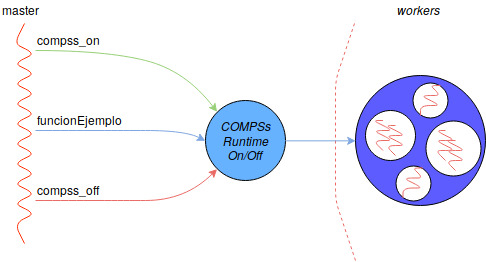
\includegraphics[width=\textwidth]{sta-masterworker.jpg}
	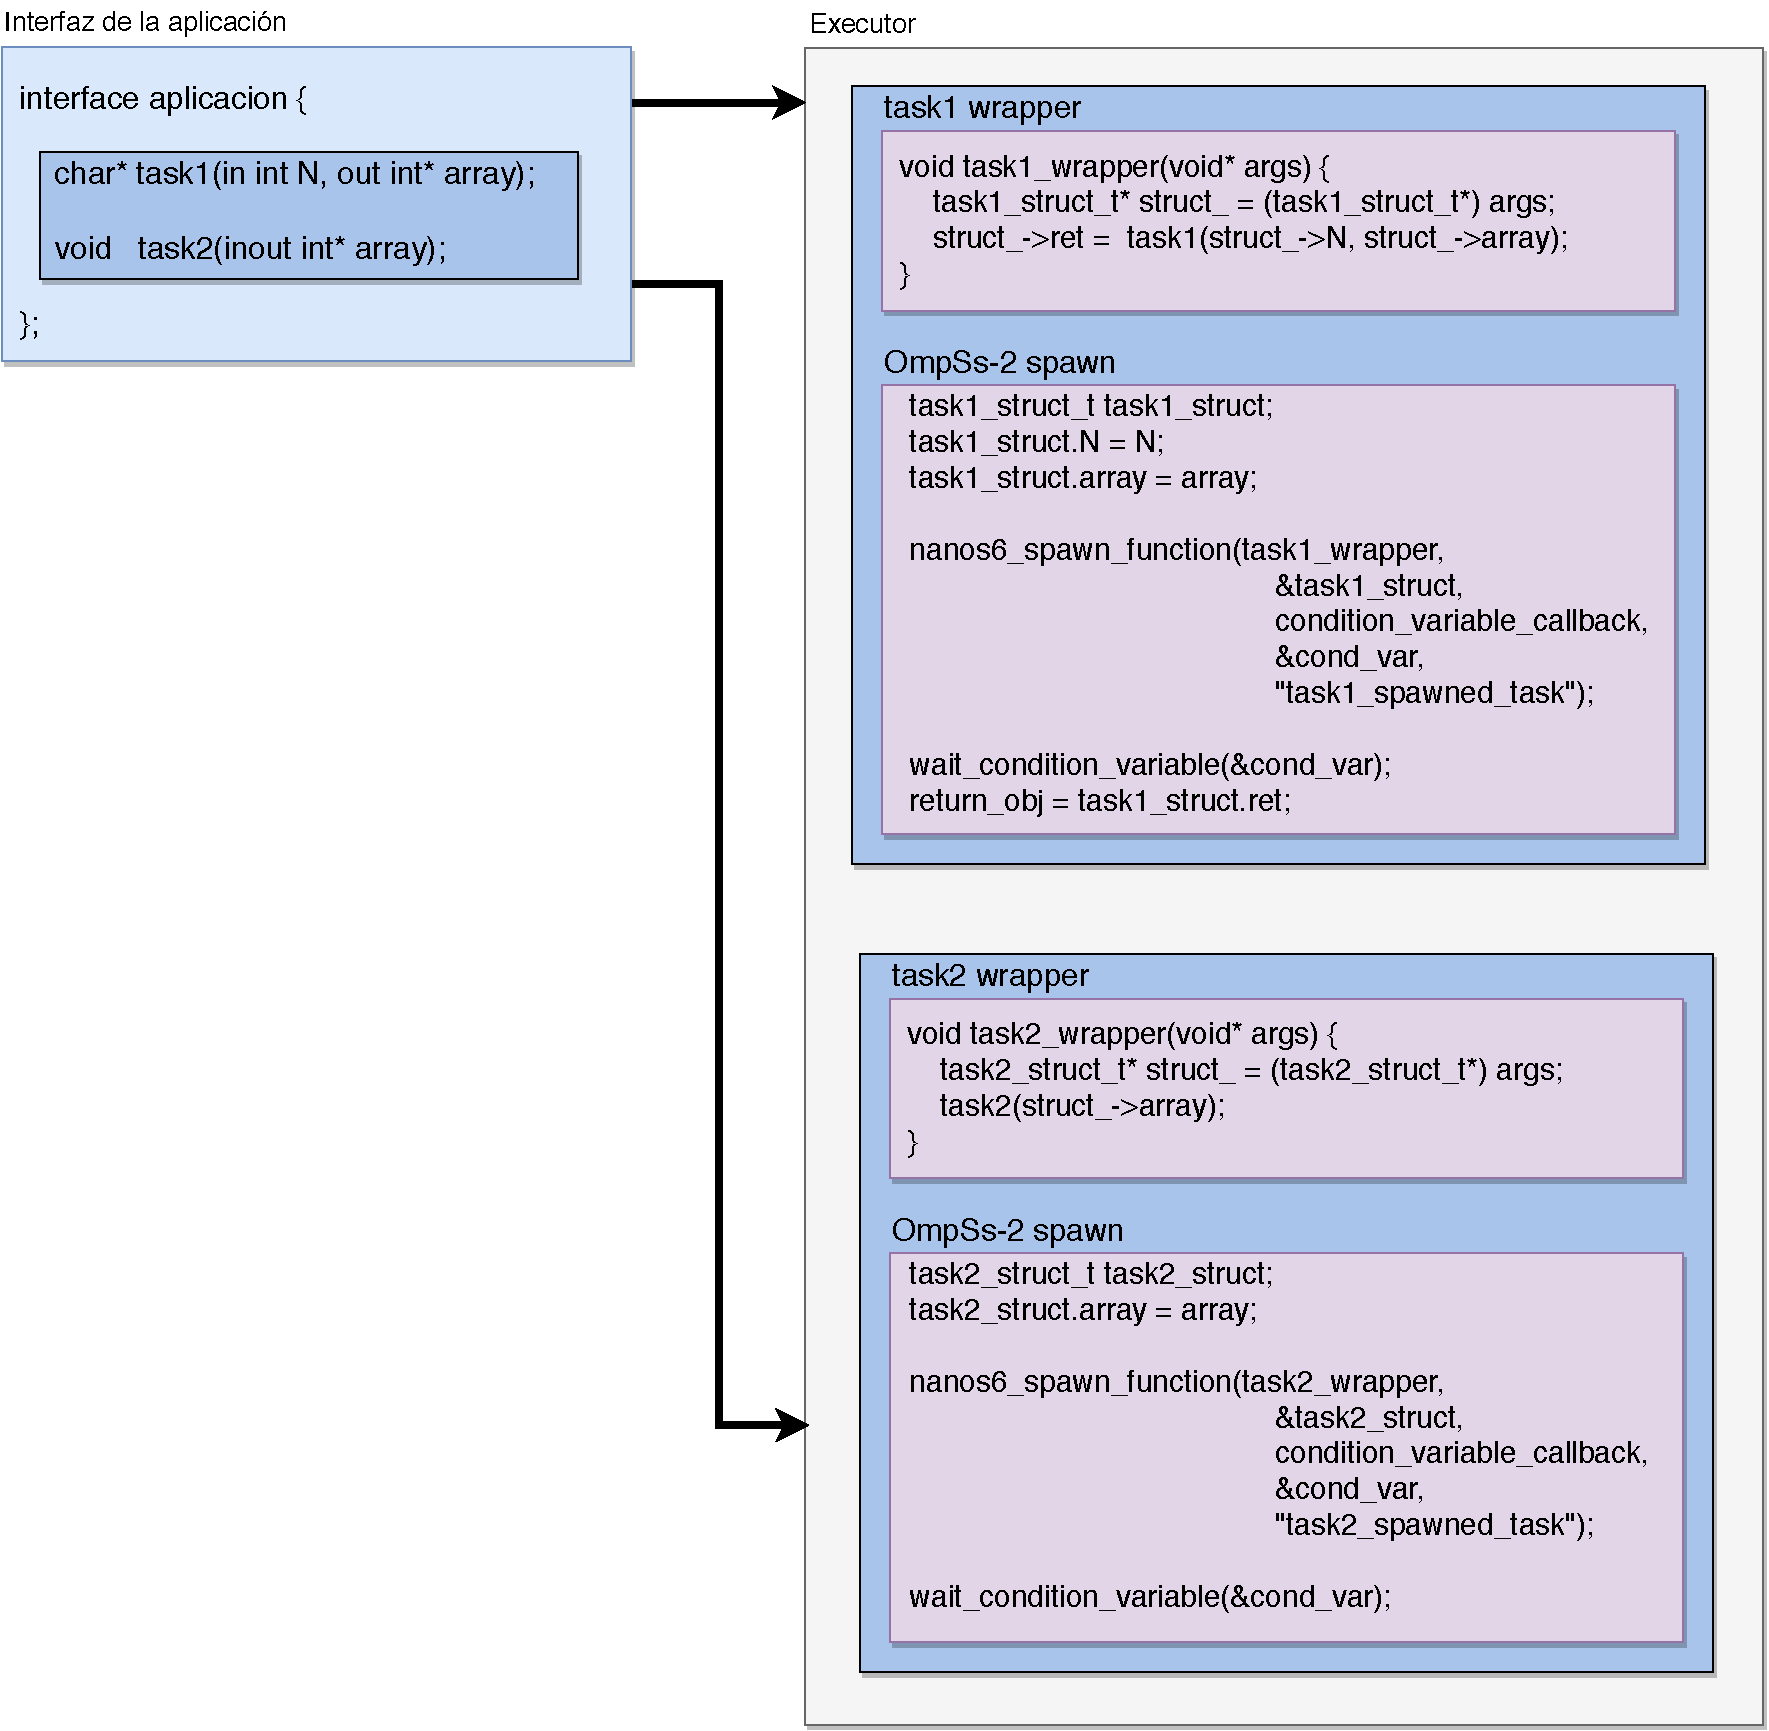
\includegraphics[scale=0.5]{generacionexecutor.pdf}
	\label{fig:genexecutorOmpSs2}
\end{figure}
\bigskip

Entonces, cada vez que al \textit{worker} se le pida ejecutar el código asociado a una tarea en concreto, si ha sido compilada para \textit{OmpSs-2} acabará pasando  por este código, de manera que se llamará al \textit{nanos6\_spawn\_function} y se ejecutará en el \textit{runtime} de \textit{OmpSs-2}. Está claro que \textit{OmpSs-2} tomará parte únicamente en los nodos del tipo \textit{worker}, ya que es donde se ejecutarán las tareas detectadas por el \textit{master}, entonces con la activación de \textit{OmpSs-2} en los nodos \textit{worker} conseguiremos la siguiente estructura y modelo de ejecución.

\par\bigskip

\begin{figure}[ht!]
    \centering 
    \caption{Estructura y modelo de ejecución master-worker de la integración COMPSs+OmpSs-2}
    %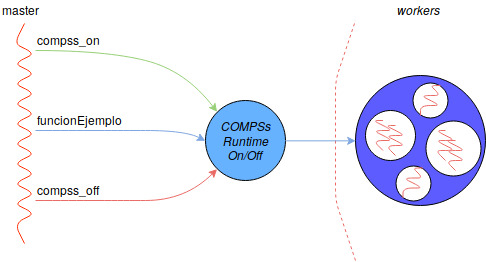
\includegraphics[width=\textwidth]{sta-masterworker.jpg}
    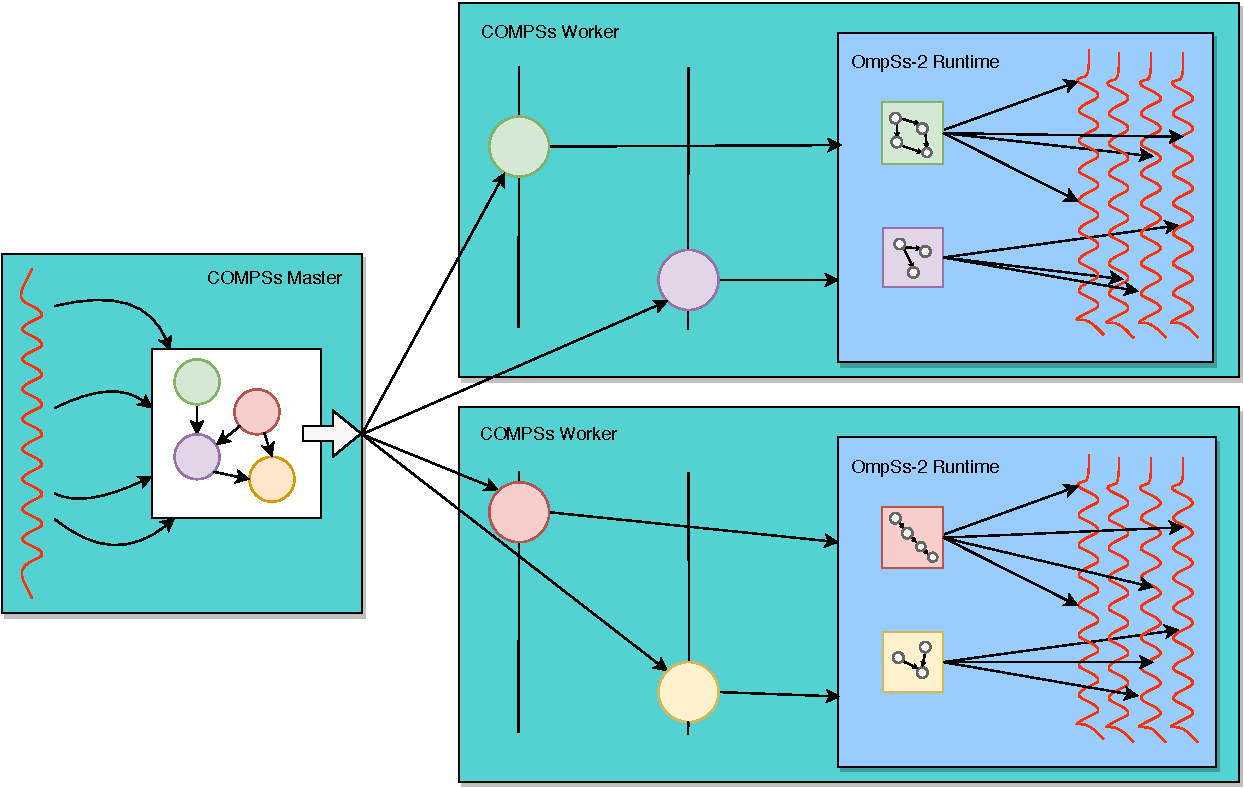
\includegraphics[scale=0.6]{compss2rt.pdf}
    \label{fig:compssompssrt}
\end{figure}

Durante la ejecución del programa principal se irá generando un grafo con las tareas que se deben ejecutar, eventualmente cada una de estas será enviada a un nodo \textit{worker} (en la figura tan sólo aparecen dos, pero podrían ser más) y este ejecutará la tarea de \textit{COMPSs} en forma de tarea de \textit{OmpSs-2}.
La ejecución de las tareas de \textit{OmpSs-2} generará otro grafo, dónde figurarán tanto las tareas que han sido creadas mediante el mecanismo de \textit{spawn} como las que puedan ser creadas dentro de las anteriores, y finalmente las tareas de este grafo serán ejecutadas. En la imagen \ref{fig:compssompssrt} se explica visualmente el modelo de ejecución, el color de las tareas de \textit{COMPSs} representa una tarea en concreto y se puede seguir su recorrido a lo largo de la ejecución.

\par\bigskip

Si juntamos la compilación y la ejecución en una sola figura resulta en la imagen \ref{fig:compejec}. A pesar que no da tantos detalles de cada componente como en las imágenes \ref{fig:workflowcompintegration} y \ref{fig:compssompssrt}, en esta imagen se ve claramente para qué se utiliza cada componente y cuál es el efecto que tiene en cada fase.

\begin{figure}[H]
	\centering 
	\caption{Fases de compilación y ejecución de una aplicación COMPSs+OmpSs-2.}
	%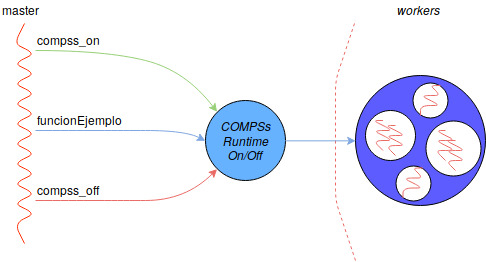
\includegraphics[width=\textwidth]{sta-masterworker.jpg}
	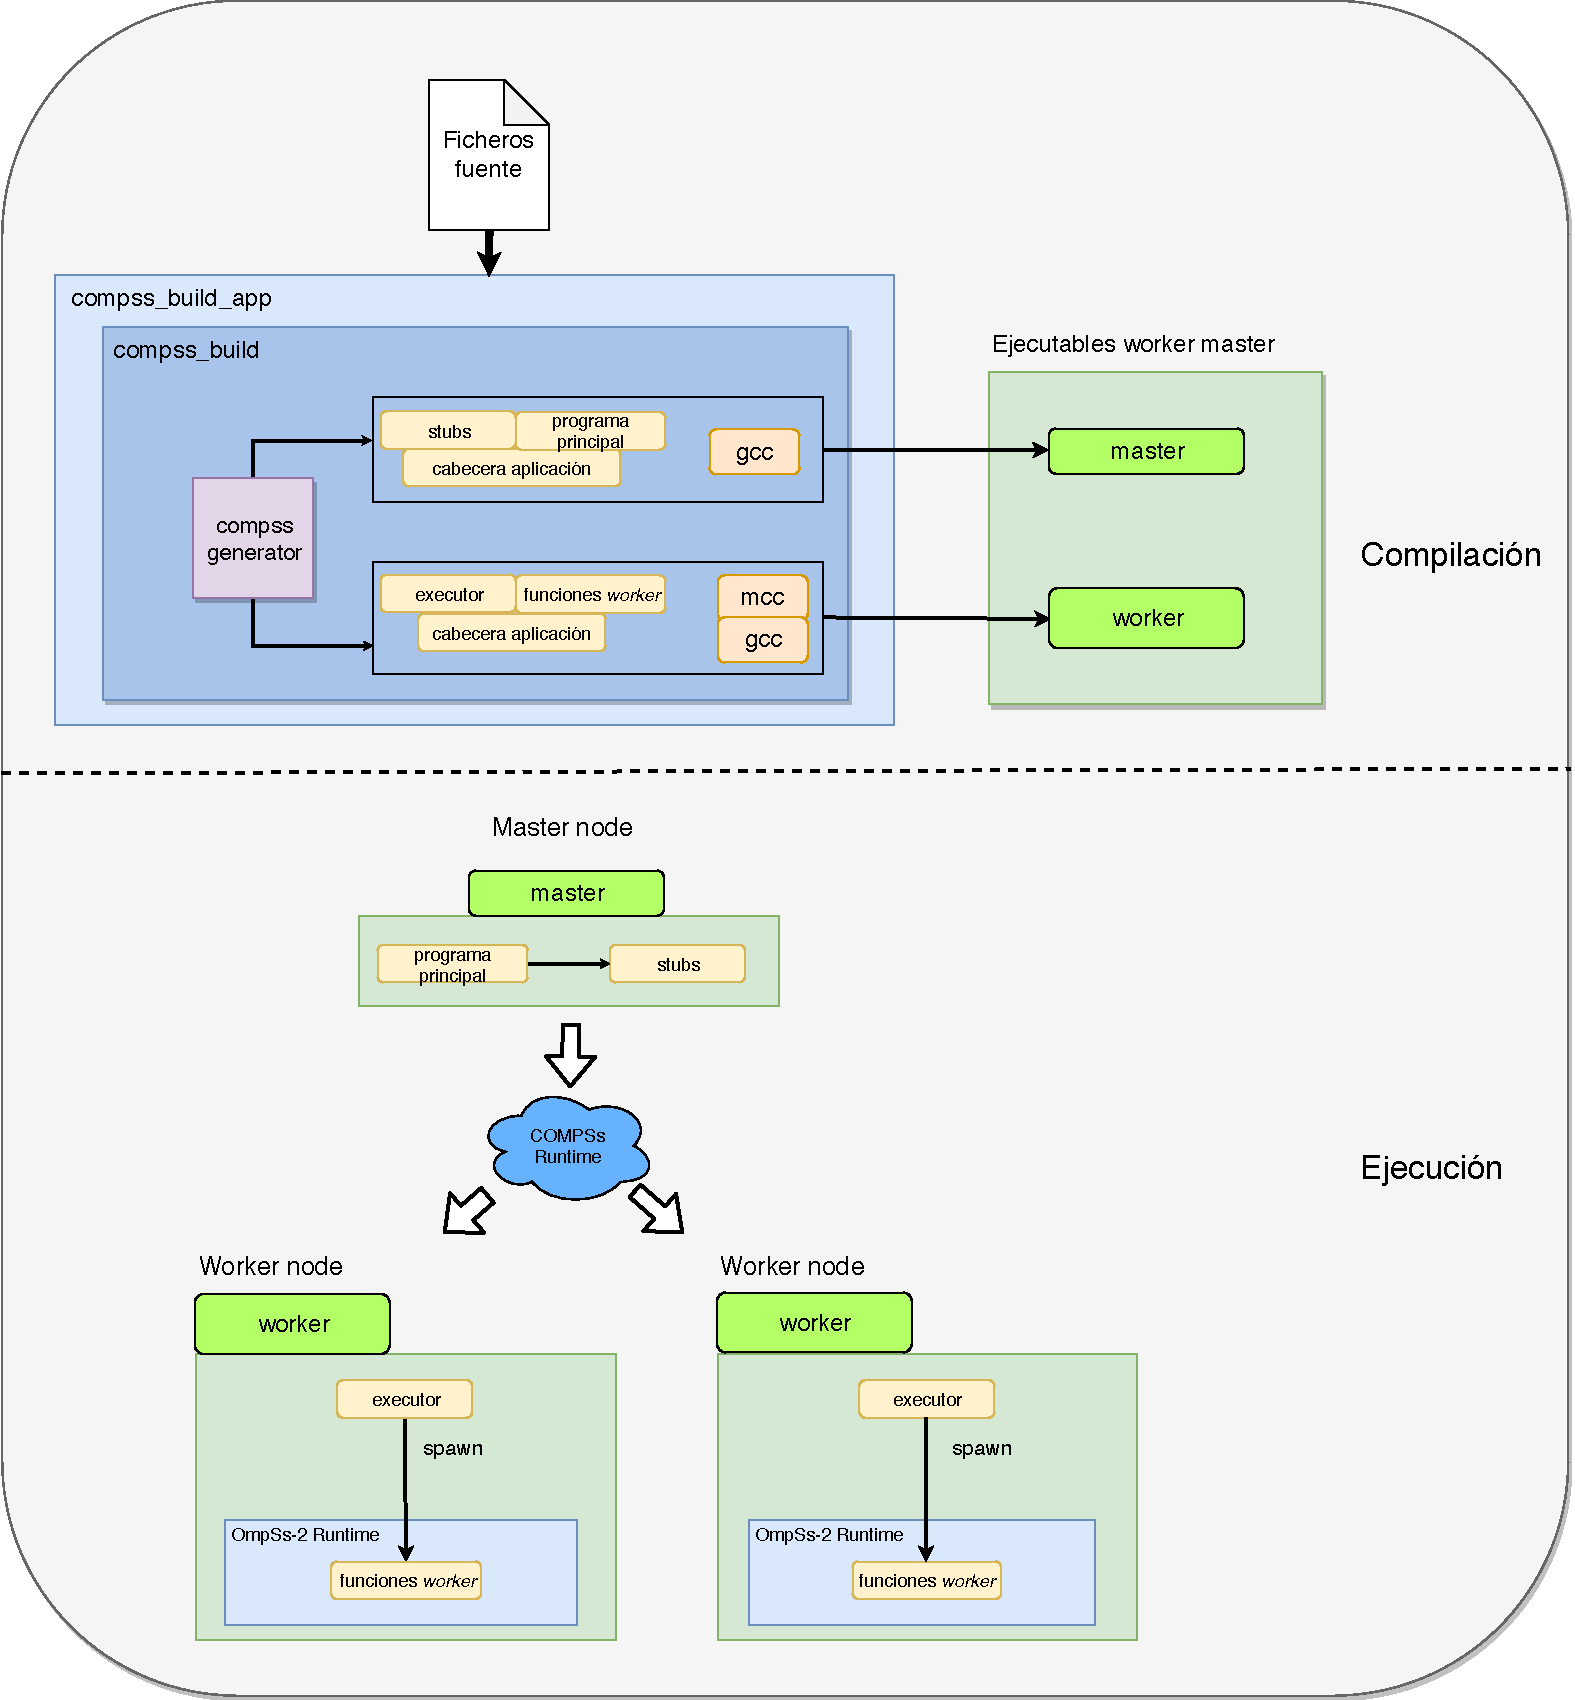
\includegraphics[scale=0.5]{compilacionplusejecucion.pdf}
	\label{fig:compejec}
\end{figure}

También en la integración se ha añadido soporte a los tipos enumerados y a la inclusión de cabeceras en la interfaz. Lo primero nos permite dar soporte a más tipos de datos y lo segundo es esencial para cuando se quieren utilizar librerías externas que requieren cabeceras. Ahora en una interfaz se puede utilizar \textit{enum} e incluir cabeceras, lo cuál se hace como en la imagen \ref{fig:enuminclude}.

\par\bigskip

\begin{figure}[H]
	\centering 
	\caption{Uso del tipo enum e incluir cabeceras en la interfaz de una aplicación.}
	%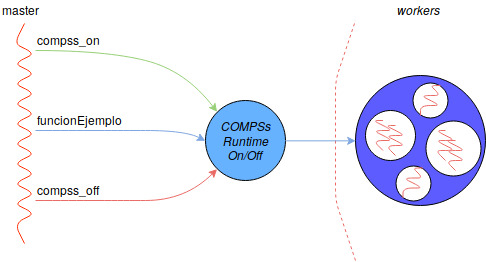
\includegraphics[width=\textwidth]{sta-masterworker.jpg}
	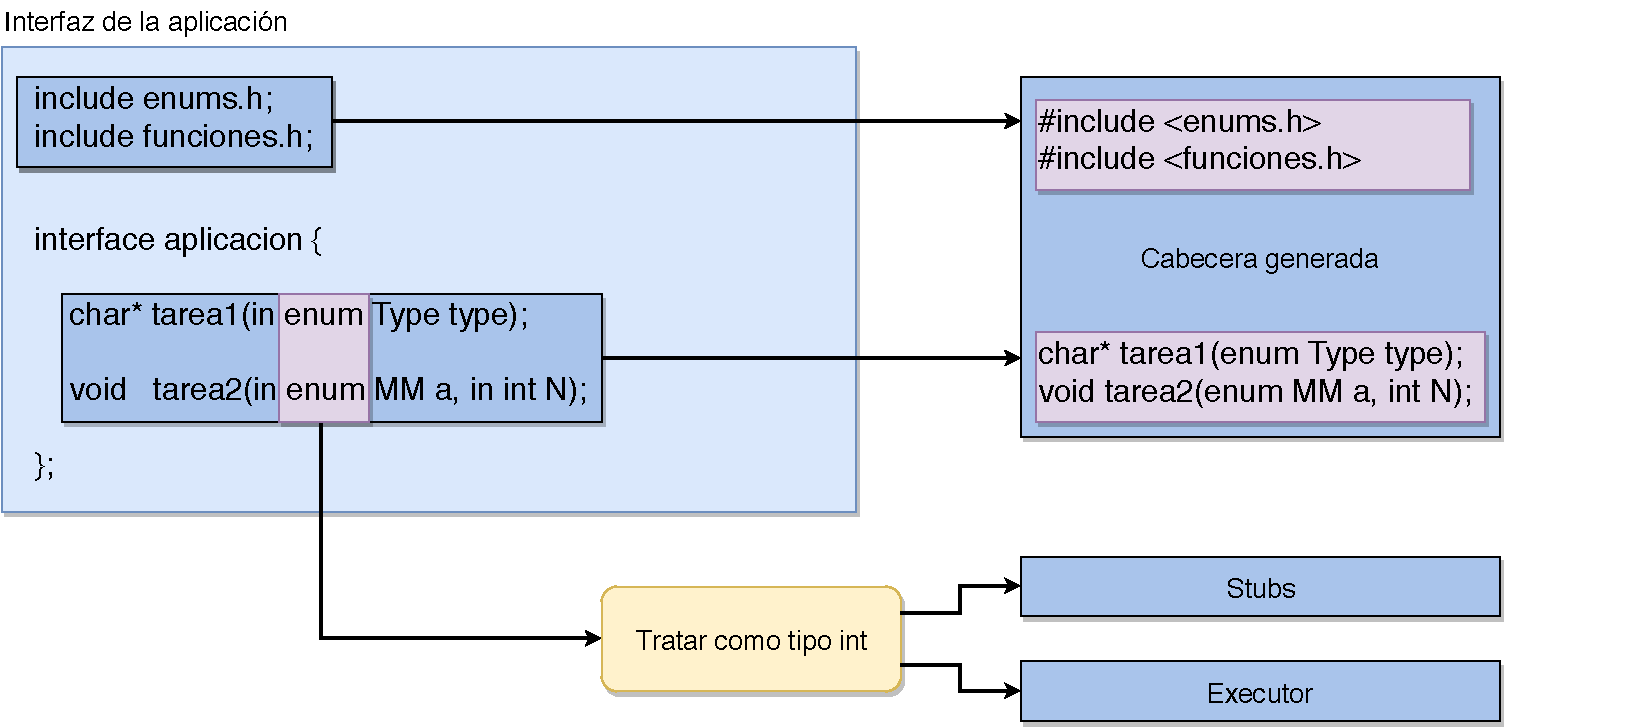
\includegraphics[scale=0.5]{enuminclude.pdf}
	\label{fig:enuminclude}
\end{figure}


\par\bigskip

Con tal de dar una explicación más sencilla, hemos evitado poner todo el código en esta sección, si se quiere más detalle o alguna parte no se entiende, en el apéndice \ref{appendix:integration} se encuentra una explicación técnica y con código de todo relativo a la integración.